
\section{Evaluation}
\label{sec:eval}

This section evaluates deterministic Linux by running compute-bound
applications using deterministic Linux and nondeterministic pthreads.
We conclude by considering a case study demonstrating the qualitative debugging
benefits of determinism.

\subsection{Empirical experiments}

Aviram et al. already demonstrated coarse-grained applications in Determinator
performed comparable to nondeterministic Linux equivalents, but fine-grained
applications did not scale nearly as well, incurring high performance costs
owing to memory synchronization costs.


\begin{table}[th]
\center{
\scalebox{.8}{
\begin{tabular}{|l| l l l l | l l l l |}
\hline
 & \multicolumn{4}{c|}{\textbf{lu}} & \multicolumn{4}{c|}{\textbf{matmult}} \\
Dimension & $N=1$ & $N=2$ & $N=4$ & $N=8$ & $N=1$ & $N=2$ & $N=4$ & $N=8$ \\
\hline
$16\times16$ & 13.1 (41.5\%) & 45.0 (46.7\%) & 46.3 (45.8\%) & 30.9 (31.5\%) &
  9.6 (48.2\%) & 21.8 (45.0\%) & 37.8 (45.2\%) & 16.0 (26.5\%) \\
$32\times32$ & 8.5 (34.0\%) & 37.3 (45.5\%) & 45.9 (46.1\%) & 29.1 (31.1\%) &
  3.3 (37.7\%) & 13.4 (42.0\%) & 21.1 (42.2\%) & 17.5 (24.1\%) \\
$64\times64$ & 2.6 (19.5\%) & 20.6 (41.6\%) & 42.1 (44.2\%) & 32.1 (30.9\%) &
  1.3 (13.4\%) & 3.8 (26.3\%) & 7.8 (34.0\%) & 13.2 (25.8\%) \\
$128\times128$ & 1.4 (2.3\%) & 6.0 (32.8\%) & 22.4 (39.0\%) & 30.8 (31.0\%) &
  1.0 (0.3\%) & 1.9 (1.7\%) & 4.5 (13.3\%) & 6.7 (18.2\%) \\
$256\times256$ & 1.1 (0.5\%) & 2.1 (11.0\%) & 7.0 (25.9\%) & 18.8 (31.1\%) &
  1.0 (0.0\%) & 1.2 (1.0\%) & 1.8 (1.6\%) & 2.3 (5.0\%) \\
$512\times512$ & 1.0 (0.1\%) & 1.2 (1.4\%) & 2.3 (9.4\%) & 5.9 (19.4\%) & 1.0
  (0.0\%) & 1.0 (0.5\%) & 1.1 (0.9\%) & 1.5 (3.0\%) \\
$1024\times1024$ & 1.4 (0.0\%) & 1.0 (0.3\%) & 1.2 (1.5\%) & 1.9 (8.4\%) & 1.0
  (0.0\%) & 0.9 (0.0\%) & 1.0 (0.1\%) & 1.2 (0.2\%) \\
$2048\times2048$ & 1.4 (0.0\%) & 1.0 (0.0\%) & 1.0 (0.1\%) & 1.1 (1.0\%) & - & - & - & - \\
\hline
\end{tabular}}}
\caption{Deterministic overhead for \emph{lu} and \emph{matmult}.
Overhead is deterministic run time divided by pthread run time.
The numbers in parentheses indicate time spent
in the kernel performing a virtual memory merge as a percentage of overall
runtime.}
\label{tab:matover}
\end{table}

\endinput



\begin{table}[t]
\center{
\scalebox{.8}{
\begin{tabular}{|l| l l l l |}
\hline
 & \multicolumn{4}{c|}{\textbf{qsort}} \\
Input size & $N=1$ & $N=2$ & $N=4$ & $N=8$ \\
\hline
1K & 27.5 & 39.2 & 24.1 & 17.4 \\
4K & 14.1 & 46.8 & 37.9 & 20.8 \\
8K & 8.6 & 28.7 & 31.4 & 23.1 \\
10K & 7.4 & 21.2 & 30.6 & 26.6 \\
40K & 2.5 & 8.4 & 13.4 & 16.8 \\
80K & 1.7 & 4.3 & 8.4 & 10.6 \\
100K & 1.6 & 3.1 & 7.6 & 11.1 \\
400K & 1.2 & 1.8 & 2.2 & 2.7 \\
800K & 1.1 & 1.4 & 1.6 & 1.6 \\
1M & 1.1 & 1.4 & 1.5 & 1.8 \\
4M & 1.1 & 1.2 & 1.3 & 1.4 \\
8M & 1.0 & 1.1 & 1.2 & 1.4 \\
10M & 1.0 & 1.0 & 1.1 & 1.3 \\
40M & 1.0 & 1.1 & 1.2 & 1.3 \\
80M & 1.0 & 1.1 & 1.2 & 1.3 \\
\hline
\end{tabular}}}
\caption{Deterministic overhead for \emph{qsort}.}
\label{tab:qover}
\end{table}

\endinput



\begin{figure}[t!]
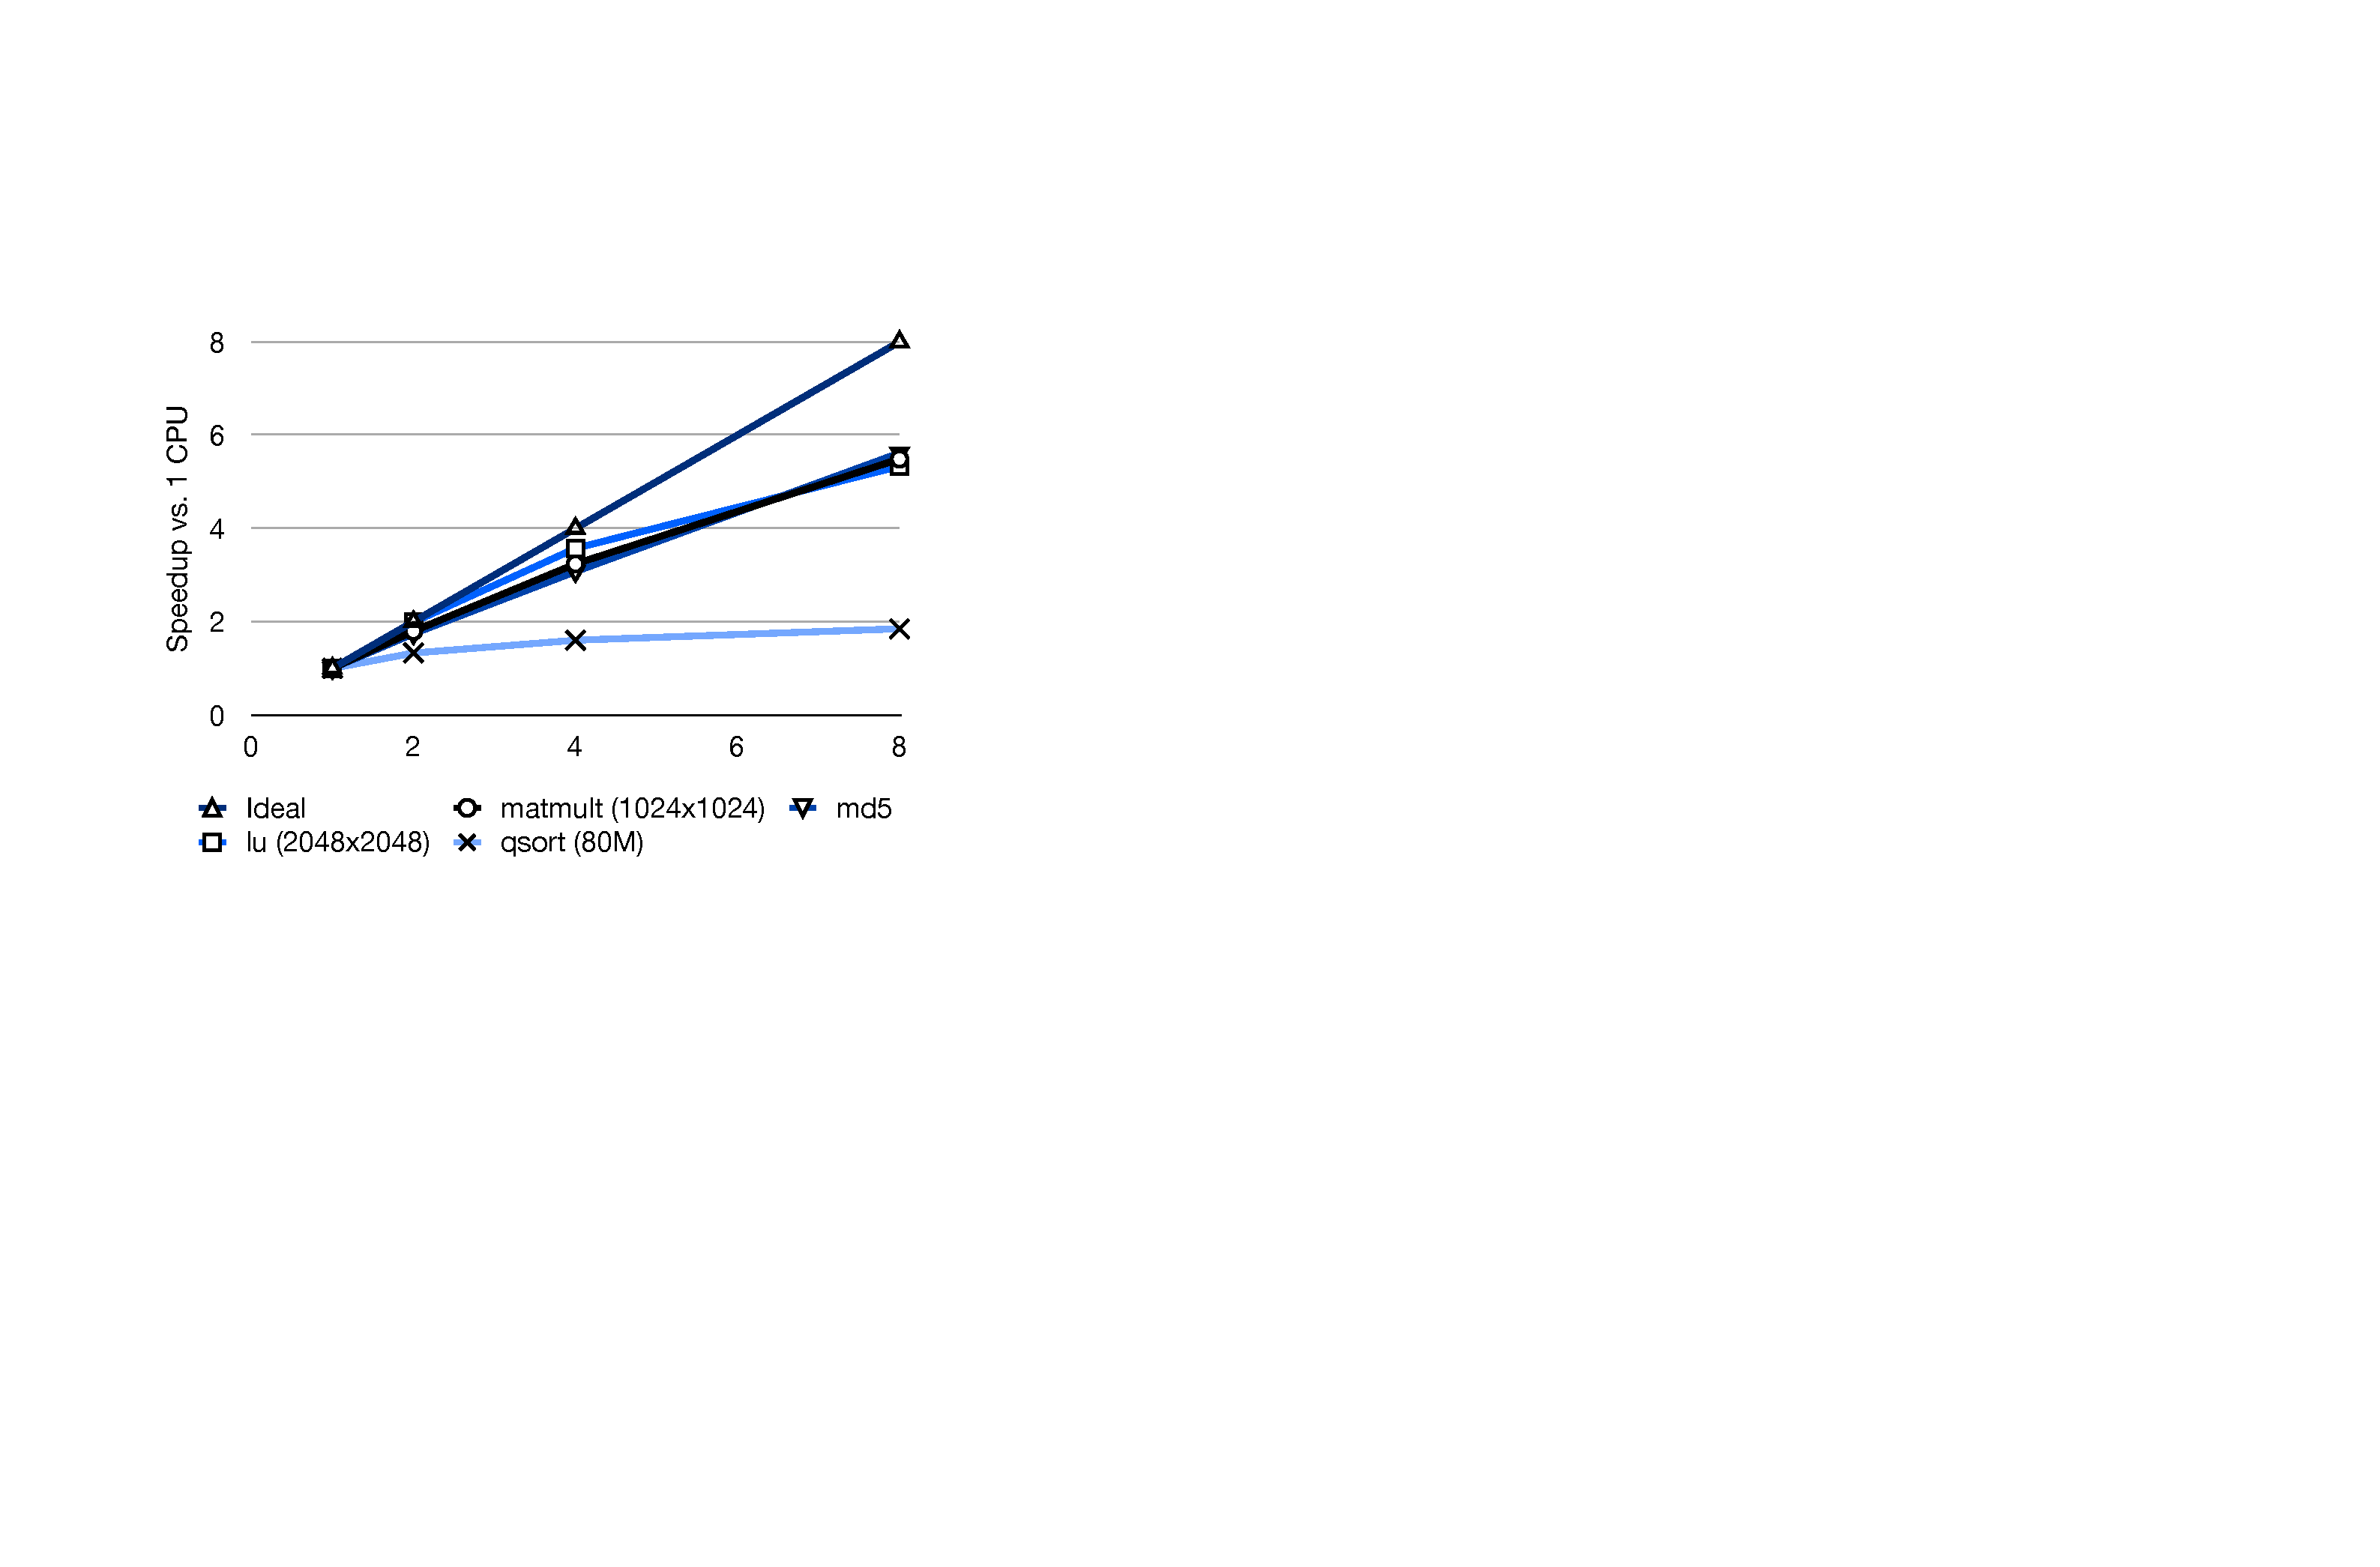
\includegraphics[scale=.45]{dspeedup.pdf}
\caption{Deterministic speedup for the parallel benchmarks.}
\label{fig:dspeedup}
\end{figure}

\endinput



The primary goal of our evaluations is to determine if Linux can efficiently run
applications using Determinator's programming model. Since the deterministic
Linux kernel reuses a lot of existing code, we expect reasonable
performance compared to the equivalent nondeterministic application. However,
applications that heavily rely on memory-intensive kernel operations like
Snapshot/Merge might incur performance penalties.

\subsubsection{Methodology}
We evaluated four benchmark programs. \emph{md5} searches for a string whose
md5 hash yields a particular hash value (i.e., a brute force password cracker).
\emph{md5} creates $N+1$ threads to perform parallel work where $N$ is the
number of processors available. The \emph{qsort} benchmark recursively sorts an
integer array by forking children threads going $log_2(2\cdot N)$ levels deep,
after which the recursive computation is carried out sequentially.
\emph{matmult} multiplies two square matrices by dividing the input into
blocks and forking off threads to multiply the individual blocks. \emph{matmult}
creates a block for each available core. \emph{lu}
performs LU decomposition of a square matrix by breaking the input into $4N^2$
blocks and creating a thread for each block.\footnote{Threads are created only
when data dependencies are satisfied. In our program, each row of blocks has a
data dependency on the row above, so at any given point in the program,
\emph{lu} creates at most $2N$ threads.}
Our LU algorithm breaks the blocks up into discontiguous blocks of memory (i.e.,
we represent our matrix in row-major order).

All benchmarks are designed so the deterministic and pthread versions operate on
identical inputs generated from a pseudorandom number generator (\emph{matult},
\emph{lu}, \emph{qsort}) or ``hardcoded'' input (\emph{md5}).
For a given input size, \emph{qsort} runs ten tests on different inputs and
averages the run times. Both matrix benchmarks run ten tests on different inputs
and average the results. \emph{md5} searches for ten fixed ASCII strings
whose values are distributed randomly over a fixed alphabet. The run times for
all ten runs are averaged to a single value, and this is done five times.

The \emph{matmult}, \emph{qsort}, and \emph{md5} benchmarks are modified
versions of benchmarks found in Determinator's source on
GitHub.\footnote{\url{https://github.com/bford/Determinator}}
The \emph{lu} benchmark was written from scratch using an algorithm described
on the Internet~\cite{lualg}. We tested on a 2 socket $\times$ 4 core 2.33 GHz
Intel Xeon PC running Arch Linux with 8GB of RAM. All benchmarks use the same
modified \mbox{x86\_64} Linux 3.0 kernel.

\subsubsection{Results}
Applications that require a lot of memory synchronization show considerable
overhead for small inputs, but have much more acceptable overheads for large
inputs.
\mbox{Table \ref{tab:matover}} shows deterministic overheads for the \emph{lu}
and \emph{matmult} benchmarks.
Execution on small inputs spends up to $48.2\%$ of their run time in the kernel
doing a memory merge.
Small inputs in general have a hard time seeing parallel benefits: the pthread
versions of both benchmarks did not see parallel speedup benefits until the
input matrix reached at least $32\times 32$ (\emph{matmult}) or $128\times 128$
(\emph{lu}). Still, it isn't until even larger
input sizes (at least $1024\times 1024$ for \emph{lu} and $256\times 256$ for
\emph{matmult}) when we begin to
see more ``acceptable'' deterministic overheads of at
most $2.3\times$.

The \emph{qsort} benchmark also shows unacceptable overhead for small inputs,
but once the input array size becomes at least 800K, overheads stayed under
$2\times$ (\mbox{Table \ref{tab:qover}}).
The embarrassingly parallel \emph{md5} benchmark exhibited very little overhead;
it had overhead of $1.16\times$ for $N=1$ and $1.05\times$ for $N=8$. This
can likely be attributed to the little amount of information transfered back and
forth between threads (a single boolean and the matching string when it is
found).

\mbox{Figure \ref{fig:dspeedup}} shows speedup over one CPU for the
deterministic benchmarks. We show the
results when run on the largest input size available
(e.g., 80M for \emph{qsort}). The \emph{md5}, \emph{lu}, and \emph{matmult}
benchmarks scale well, and \emph{qsort} scales poorly, not even
reaching $2\times$ when $N=8$. \mbox{Figure \ref{fig:scale}} compares
scalability of the pthreads benchmarks against the deterministic versions.
In all four benchmarks, we see that the deterministic programs have about the
same ability to scale as the pthread programs. For \emph{lu} and \emph{md5},
the deterministic versions scale better due to high overheads in the $N=1$
case that diminish as we add more CPU cores.

\subsubsection{Fine-tuning the benchmarks}
\label{sec:finetune}
We may attribute some of the exceptionally high overhead for small inputs to
the cost of merging. For simplicity, our deterministic thread join merges the
entire static data segment. \emph{qsort}, \emph{matmult}, and \emph{lu} all
declare static arrays with sizes as large as the maximum expected input. For
example, \emph{lu} declares two {\tt long double} arrays of size
$2048\times 2048$ for a total of 128MB on our 64-bit machine. When we join on
all 256 threads for the $16\times 16$ input, we merge over all 128MB. Page
table optimizations (Section \ref{sec:memop}) enable the kernel to only have to
do a \mbox{byte-by-byte} merge for the single page containing the input matrix,
but the kernel must still check at least 32767 other page table
entries for each merge!\footnote{Assuming 4KB pages.}

Thankfully, the syscall API allows us to specify a range of virtual memory to
merge; we could fine-tune our programs to merge only what we know has changed.
For the \emph{qsort} benchmark, we could opt to use the {\tt Copy} option to
achieve the same effect. {\tt Copy} copies page tables directly without checking
page table entries and possibly the bytes themselves as {\tt Merge} does. By
having our high-level join function merge the entire static data segment, our
join method is very general in the types of programs it can be used with. We
could likely trade this generality for performance gains.


\begin{figure*}[t]
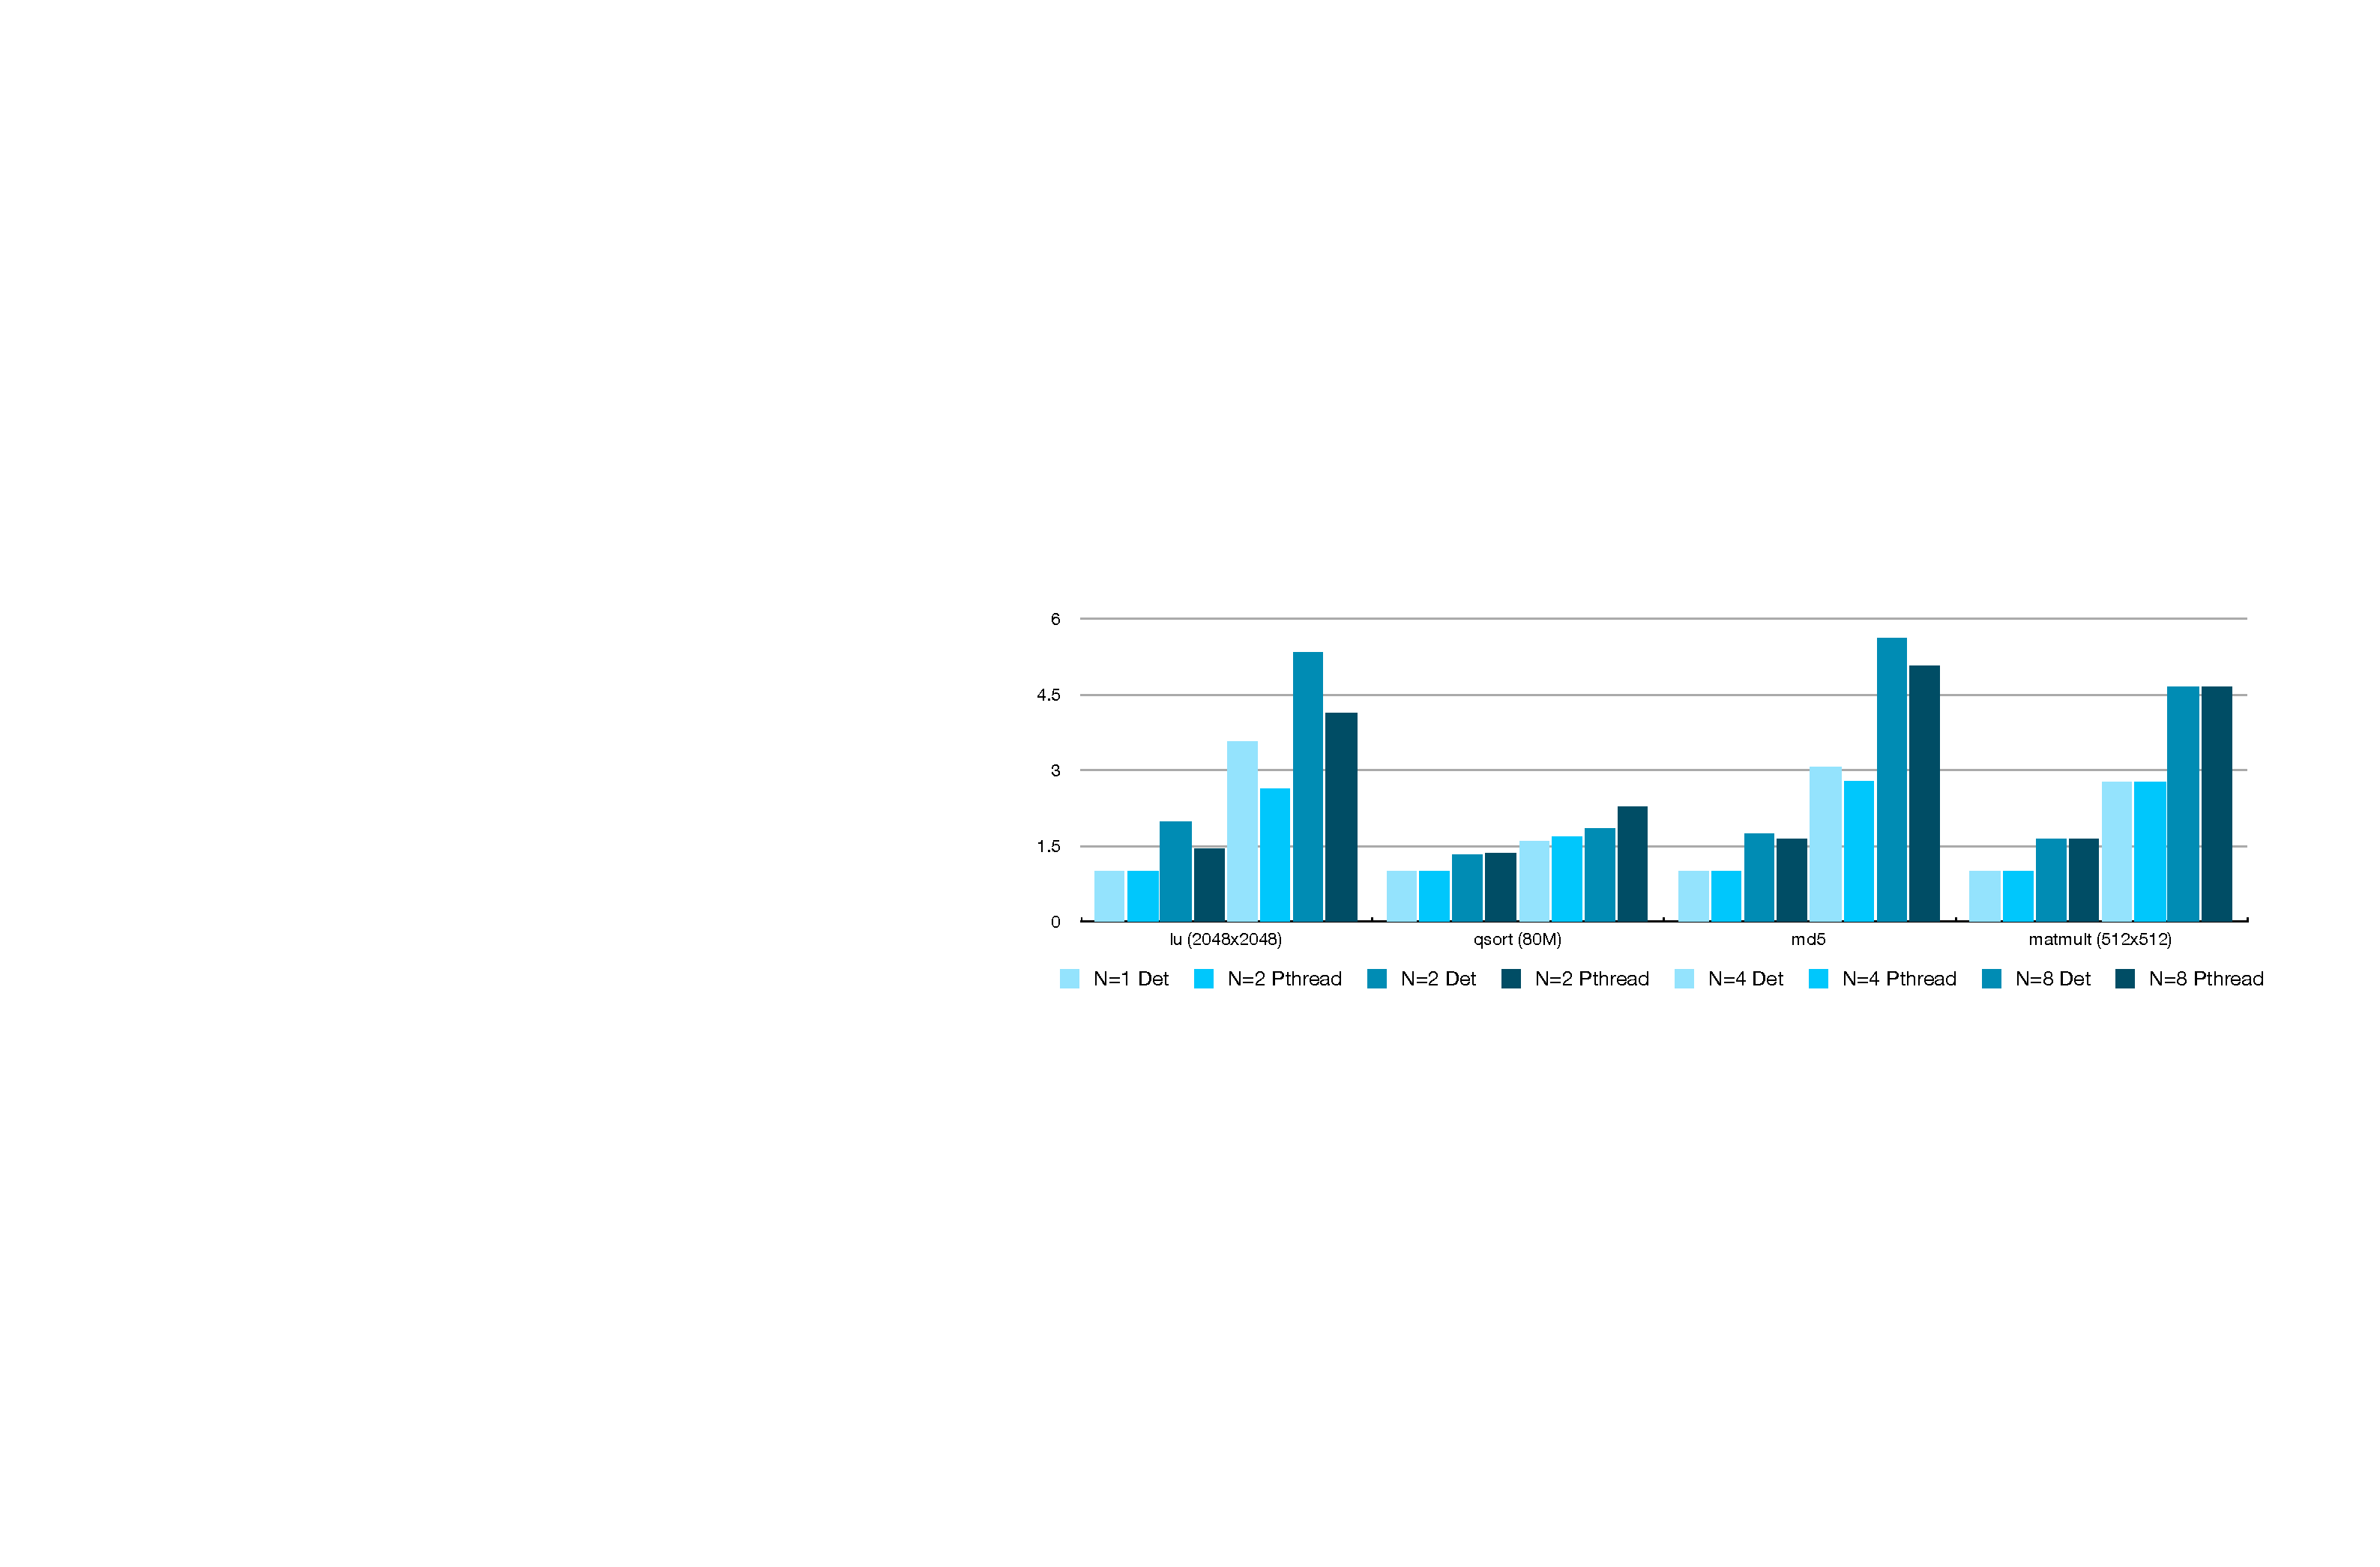
\includegraphics[scale=.59]{scale.pdf}
\caption{Comparing the speedup over $N=1$ for the deterministic and pthread
versions of the benchmarks. This figure demonstrates the ability of both
versions to scale as we add more CPU cores.}
\label{fig:scale}
\end{figure*}

\endinput



\subsubsection{Qualitative evaluation}
This section attempts to give a qualitative understanding of how the benchmarks
work. Each of our benchmarks uses the fork/join paradigm. The pthread
applications fork and join threads with \mbox{\tt pthread\_create()} and
\mbox{\tt pthread\_join()}. The deterministic benchmarks create threads by
issuing a {\tt dput()} specifying the {\tt Snap} option; we join thread results
by performing a {\tt Merge} on the
program's entire static data segment (initialized and uninitialized). At the
kernel level, creating deterministic threads incurs the additional cost of
creating two copies of the parent's page tables and associated kernel data
structures. Since pthreads threads share memory, the kernel merely
copies a pointer to the parent's memory management structure to the child.
Joining blocks the parent thread until the child finishes execution. The
deterministic join, however, incurs the cost of merging a potentially large
region of memory.

We should also consider an otherwise overlooked overhead associated with
copy-on-write. When a deterministic child thread writes to page marked COW,
the kernel intervenes to allocate a new page, copy the page contents, and
invalidate at least one TLB entry.\footnote{TLB invalidation is a costly
operation, especially if the CPU only supports invalidating the entire TLB.}
In fact, tracing through the page fault code and manually counting the number of
semicolons gives a conservative estimate of 84. A similar trace through
Determinator's COW code counts only 23 semicolons.
Thus, for all inputs, and especially the smaller input sizes, we suspect
that COW contributes a nontrivial amount of overhead.

\subsection{Finding bugs deterministically}

To demonstrate one of the key benefits of deterministic execution (Section
\ref{sec:det-motiv}), we consider a Gaussian elimination program written using
the deterministic API and pthreads. Figures \ref{fig:pgauss} and
\ref{fig:dgauss} show nondeterministic and deterministic portions of Gaussian
elimination code. There is a crucial synchronization bug, however: both
algorithms create \mbox{\tt nrows - k} worker threads but only join
\mbox{\tt nrows - k - 1} threads. We purposefully inserted this bug, but the
reader can imagine a programmer making this typo by mistake.


\begin{subfigures}
\begin{figure}[t!]
{\tt \footnotesize
\begin{verbatim}
pthread_t thread[MAXTHREADS];
struct thread_data data[MAXTHREADS];
void pthread_reduce(void) {
   for (i = 1; k <= nrows - 1; ++k) {
      for (i = k + 1; i <= nrows; ++i) {
         data[i] = /* Setup worker. */;
         pthread_create(&thread[i], NULL, worker,
            &data[i]);
      }

      /* Bug! Should be i <= nrows */
      for (i = k + 1; i < nrows; ++i)
         pthread_join(thread[i], NULL);
   }
}
\end{verbatim}
}
\caption{pthread Gaussian elimination.}
\label{fig:pgauss}
\end{figure}
\begin{figure}[th!]
{\tt \footnotesize
\begin{verbatim}
/* Forks a deterministic child. Returns 0 into the
 * child and 1 into the parent. */
int dfork(pid_t childid);
/* Merges a child's changes into the parent after
 * the child issues a dret(). */
void djoin(pid_t childid);

void det_reduce(void) {
   for (i = 1; k <= nrows - 1; ++k) {
      for (i = k + 1; i <= nrows; ++i) {
         data[i] = /* Setup worker. */;
         if (!dfork(i)) { worker(&data[i]); dret(); }
      }

      /* Bug! Should be i <= nrows */
      for (i = k + 1; i < nrows; ++i)
         djoin(i);
   }
}
\end{verbatim}
}
\caption{Deterministic Gaussian elimination.}
\label{fig:dgauss}
\end{figure}
\end{subfigures}

\endinput



We ran both versions multiple times and examined the resulting matrix.
The deterministic program \emph{always}
produced the wrong answer. {\tt djoin()} merges changes back into the main
thread for all but the last worker thread. When the last worker thread
finishes, its changes are private and never seen by the main thread.

On the other hand, the pthreads program executes nondeterministically. We
observed three different output matrices, one of which was the correct result.
If the final worker thread finishes before we observe the final result, the
output will be correct. If the final worker thread does not finish by the time
we examine the output, we get an intermediate result. The output is
nondeterministic, owing to a race condition, since all threads share memory.

Determinism provides a clear benefit in debugging, since the deterministic
version always behaves the same, whereas the buggy behavior might exhibit itself
rarely in the pthread version.
We also consider testing our application to ensure its correctness.
When testing our Gaussian elimination application, determinism allows us to see
right away that, in general, all inputs give incorrect answers. On the other
hand, it may be the case that the nondeterministic version always gives
the correct answer for matrices we test on a development machine, but as soon as
we ship the program to a client's machines with a different number of processors
(for example), the bug exhibits itself.

\endinput

